\newpage 
\chapter{مقدمه}
\label{ch:intro}


مساله‌ی یافتن نمایش تنک\LTRfootnote{Sparse Representation }
سیگنال‌ها در یک دیکشنری فوق کامل \LTRfootnote{Over Complete }
یا به صورت معادل یافتن تنک‌ترین پاسخ یک دستگاه معادلات خطی فرومعین\LTRfootnote{Under Determined }
، یعنی دستگاهی که در آن تعداد معادلات از تعداد مجهولات کمتر است، در سال‌های اخیر محور توجه بسیاری از تحقیقات انجام شده در حوزه‌ی پردازش سیگنال دیجیتال بوده است. در این سال‌ها پیشرفت چشم‌گیری در رابطه با حل این مساله و کاربرد‌های آن حاصل شده است
\cite{candes2006robust,donoho2006compressed,donoho2006stable,donoho2006most}. 
در حقیقت، حل این مساله	 در بسیاری از حوزه‌های مطرح دنیای پردازش سیگنال دیجیتال همچون جداسازی کور منابع\LTRfootnote{Blind Source Sepereation }\cite{gribonval2006survey}
، حسگری فشرده\LTRfootnote{Compressed Sensing }
یا نمونه‌برداری فشرده\LTRfootnote{Compressive Sampling }
\cite{candes2006compressive,donoho2006compressed}
و نیز در بسیاری از کاربرد‌های مخابراتی همچون تخمین کانال
\cite{carbonelli2007sparse}
مخابرات چند کاربره بر اساس 
\lr{CDMA}
\cite{aktas2003single,angelosante2010sparsity}
و سیستم‌های چند آنتنی
\cite{dongming2003channel}
کاربرد دارد. همچنین کاربرد‌های فراوانی از این شاخه‌ی نظری پردازش سیگنال دیجیتال در زمین‌شناسی، علوم زیستی و علوم فضایی گزارش شده است.

از طرف دیگر، در سیستم‌های عملیاتی امکان دقت بی‌نهایت در نمونه‌ها وجود ندارد.

\section{مقدمه‌ای بر حسگری فشرده}
در بسیاری از مسایل علمی و تکنولوژی، یک مساله‌ی مهم، دریافت اطلاعات از نمونه‌های دریافتی است. برای مثال، در پردازش سیگنال یا تصویر، هدف بازیابی سیگنال اصلی با استفاده از نمونه‌های دریافتی است. در حالتی که روند دریافت اطلاعات خطی باشد، استخراج اطلاعات در واقع برابر با حل یک دستگاه معادلات خطی است. به عبارت ریاضی، داده‌های مشاهده شده‌ی 
$\bm{y}\in \R^{m}$
به سیگنال مورد نظر 
$\bm{x}\in \R^{N}$
توسط رابطه‌ی 
\begin{align}
\label{eq:eq1}
\bm{y}=\bm{A}\bm{x}
\end{align}
مرتبط می‌شود. در رابطه‌ی
\eqref{eq:eq1}
ماتریس
$\bm{A}\in \R^{m\times N}$
، ماتریس اندازه‌گیری خطی و مدل کننده‌ی  فرآیند نمونه‌برداری است. جهت به دست آوردن سیگنال 
$\bm{x}$
از رابطه‌ی فوق، اولین راهی که به نظر می‌رسد، حل دستگاه معادلات خطی است. در روش‌های سنتی،‌ جهت حل دستگاه معادلات،  تعداد نمونه‌های اخذ شده 
$(m)$
باید حداقل برابر با بعد سیگنال مجهول 
$(N)$
(تعداد درایه‌های بردار 
$\bm{x}$
) و یا بیشتر باشد. این فرض به عنوان یک شرط پایه‌ای در بسیاری از تجهیزات موجود همانند مبدل‌های آنالوگ به دیجیتال 
\lr{(ADC)}\LTRfootnote{analog-to-digital converter}
تجهیزات تصویربرداری پزشکی، رادار و ارتباطات بیسیم،‌ در نظر گرفته می‌شود. در واقع در حالتی که 
$m<N$
است، در جبر خطی سنتی، دستگاه معادلات خطی 
\eqref{eq:eq1}
، فرومعین\LTRfootnote{underdetermined}
نامیده می‌شود و در حالت کلی در صورتی که بتوان یک پاسخ برای آن پیدا نمود مساله بینهایت پاسخ خواهد داشت.  به عبارت دیگر، بدون اطلاعات اضافی دیگر، بازیابی سیگنال 
$\bm{x}$
با استفاده از نمونه‌های
$\bm{y}$
در حالتی که 
$m<N$
باشد، امکان‌پذیر نخواهد بود. این موضوع، از طرف دیگر به قضیه‌ی نمونه‌برداری شانون-نایکوییست
\LTRfootnote{Shannon-Nyquist  sampling theorem}
مرتبط است که در آن جهت تضمین بازیابی اطلاعات، نرخ نمونه‌برداری باید حداقل برابر با دو برابر بیشترین فرکانس موجود در سیگنال باشد.


به این ترتیب، بازیابی سیگنال با استفاده از یک دستگاه معادلات خطی فرومعین بسیار جذاب خواهد بود. فرض اساسی که منجر به حل این دستگاه می‌شود 
\textbf{تنکی}\LTRfootnote{Sparsity}
است. حوزه‌ی تحقیقاتی که به تحلیل تئوری و ارائه‌ی الگوریتم در این زمینه می‌پردازد، حسگری فشرده\LTRfootnote{Compressed sensing}
، نمونه‌برداری فشرده\LTRfootnote{Compressive samplin}
یا بازیابی تنک\LTRfootnote{Sparse recovery}
نام دارد. 

در صورتی که بیشتر درایه‌های یک سیگنال صفر باشد، آن سیگنال تنک نامیده می‌شود. مشاهدات تجربی نشان می‌دهد که بسیاری از سیگنال‌های حقیقی، فشرده‌پذیر یا به صورت تقریبی تنک هستند. این سیگنال‌ها یا به صورت مستقیم تنک هستند و یا بعد از تغییر مناسب در پایه‌های توصیف کننده تنک می‌گردند. الگوریتم‌های فشرده‌سازی تصویر بر مبنای این حقیقت بنا شده است. به عنوان مثال، در 
\lr{JPEG}
تصویر پس از اعمال تبدیل 
\lr{DCT}
یا موجک تنک می‌گردد. برای فشرده‌سازی تصویر در این روش ابتدا مقادیر پایه‌ها بر اساس دامنه به صورت نزولی مرتب می‌شوند و در ادامه مولفه‌هایی که مقدار آنها کم است، صفر قرار داده می‌شود. اگرچه معمولا تعداد زیادی از پایه‌ها صفر می‌گردد ولی در تصویر بازیابی شده در این حالت تغییر محسوسی حس نمی‌گردد.

با اضافه نمودن فرض تنکی یا فشرده‌پذیری سیگنال، در مساله‌ی بیان شده، رویکرد سنتی دریافت نمونه‌های زیاد نوعی انباشت اطلاعات زائد به نظر می‌رسد. به عبارت دیگر با این روش نمونه‌برداری، سعی در بازیابی تعداد زیادی صفر در سیگنال مورد بررسی داریم. در حسگری فشرده با فرض تنکی، سعی در بازیابی سیگنال فشرده‌پذیر با تعداد نمونه‌های اندک داریم. دشواری اصلی در حسگری فشرده پیدا کردن محل درایه‌های غیر صفر در سیگنال 
$\bm{x}$
است. 


به صورت شهودی، اطلاعات ذاتی یک سیگنال فشرده‌پذیر از طول سیگنال بسیار کمتر است (در غیر این صورت فشرده‌سازی امکان‌پذیر نخواهد بود). بدیهی است که تعداد نمونه‌های دریافتی از یک سیگنال باید به حدی باشند که بتوان این اطلاعات ذاتی را استخراج نمود. با این وجود بازیابی سیگنال در این حالت به سادگی روش‌های قدیمی نیست. 

تئوری حسگری فشرده در پی پاسخ به دو سوال اساسی زیر است.
\begin{itemize}
\item{
فرآیند نمونه‌برداری خطی چگونه طراحی گردد؟ به عبارت دیگر ماتریس 
$\bm{A}$
چه شرایطی باید داشته باشد.
}
\item{
چگونه 
$\bm{x}$
از
$\bm{y}=\bm{A}\bm{x}$
بازیابی گردد؟
به عبارت دیگر الگوریتم بازیابی مناسب چگونه است.
}
\end{itemize}

دو سوال مطرح شده به طور کامل بی ارتباط نیستند و الگوریتم بازیابی نیازمند ماتریس 
$\bm{A}$
است اما می‌توان ماتریس 
$\bm{A}$
را به صورت جداگانه از الگوریتم تحلیل نمود.

نتایج حسگری فشرده به ازای هر ماتریس اختیاری 
$\bm{A}$
برقرار نیست. به عنوان مثال اگر ماتریس 
$\bm{A}$
را ماتریس قطری مستطیلی در نظر بگیریم،‌ در نمونه برداری به صورت
$\bm{y}=\bm{A}\bm{x}$
تنها چند مولفه از بردار 
$\bm{x}$
را انتخاب نموده‌ایم که با توجه به تنک بودن بردار 
$\bm{x}$
بیشتر این مقادیر صفر خواهند بود و هیچ اطلاعاتی در رابطه با محل درایه‌های غیر صفر اخذ نشده است. با انتخاب چنین ماتریسی بازیابی سیگنال غیر ممکن خواهد بود. بنابراین حسگری فشرده تنها در الگوریتم‌های بازیابی خلاصه نمی‌گردد. درایه‌های ماتریس اندازه‌گیری باید مستقل از سیگنال ورودی و ثابت باشند. منظور از ثابت بودن درایه‌های ماتریس این است که مقادیر آن غیر وفقی و مستقل از مقدار ورودی در نظر گرفته شود. 

در کاربرد‌های عملی، در دسترس بودن یک الگوریتم با سرعت منطقی جهت بازیابی سیگنال ضروری است. این ویژگی سبب شده که توجه بسیار زیادی معطوف حسگری فشرده گردد. با توجه به خواص بیان شده، اولین الگوریتمی که به ذهن خطور می‌کند، کمینه‌سازی نُرم صفر است. در طول این پایان‌نامه  نماد 
$\norm{\bm{x}}_{0}$
نشانگر تعداد درایه‌های غیر صفر بردار
$\bm{x}$
است. با این فرض، پاسخ بهینه‌سازی زیر به عنوان سیگنال بازیابی شده در نظر گرفته می‌شود.
\begin{align}
\label{eq:eq2}
\min \norm{\bm{z}}_{0} \quad \text{s.t.}\quad \bm{y}= \bm{A}\bm{z}
\end{align}

در مساله‌ی بهینه‌سازی فوق، ما به دنبال تنک‌ترین بردار 
$\bm{z}$
هستیم که در شرط 
$\bm{y}= \bm{A}\bm{z}$
صدق می‌کند. متاسفانه مساله‌ی کمینه‌سازی نُرم صفر در حالت کلی 
 \lr{NP}-سخت
 است و یافتن پاسخ در ابعاد بالا امکان‌پذیر نیست. جهت بازیابی از نسخه‌ی رها شده \LTRfootnote{Relaxed}
 مساله‌ی کمینه‌سازی نُرم صفر با نام پیگیری پایه‌ها
\LTRfootnote{Basis pursuit}
 یا کمینه‌سازی نُرم یک استفاده می‌شود. مساله‌ی پیگیری پایه‌ها به صورت زیر تعریف می‌گردد.
\begin{align}
\label{eq:eq3}
\min \norm{\bm{z}}_{1} \quad \text{s.t.}\quad \bm{y}= \bm{A}\bm{z}
\end{align}
در رابطه‌ی فوق
$\norm{\bm{z}}_{1}$
به صورت 
$\Sigma_{i} |z_{i}|$
تعریف می‌گردد. با توجه به اینکه نُرم 
\lr{$\ell_{1}$}
یک تابع محدب است، مساله‌ی بهینه‌سازی 
\eqref{eq:eq2}
با استفاده از روش‌های بهینه‌سازی محدب به سادگی قابل حل است. البته نُرم به ازای مقادیر بیشتر از یک نیز محدب است. در شکل
\ref{fig1}
توپ واحد نُرم به ازای مقادیر مختلف نمایش داده شده است. در حالت کلی نُرم
$\ell_{p}$
به صورت
$\norm{x}_{p}= \left(\Sigma_{i} |x_{i}|^{p} \right)^{1/p}$
تعریف می‌گردد.
\begin{figure}[t]
\centering
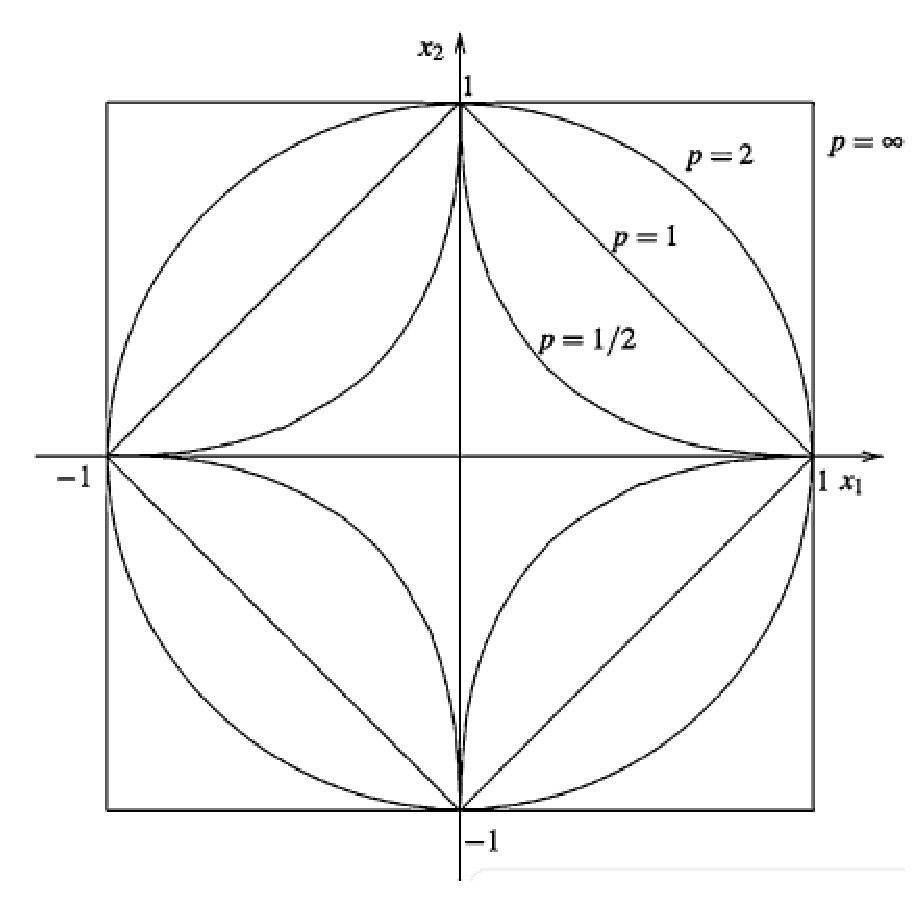
\includegraphics[scale=0.3]{Images/ch1/fig1.eps}
\caption{توپ واحد نُرم $l_{p}$ به ازای مقادیر مختلف $p$}
\label{fig1}
\end{figure}

اگر بجای استفاده از نُرم 
$\ell_{1}$
از نُرم
$\ell_{2}$
 استفاده کنیم، میزان خطا در بازیابی به شدت افزایش می‌یابد. با توجه به شکل
\ref{fig2}
علت این خطا کاملا مشهود است. همانگونه که از شکل مشخص است به ازای نُرم دوم پاسخ محاسبه شده لزوما تنک نیست که با فرض مسأله در تناقض است
\cite{boche2015compressed}.

\begin{figure}
\centering
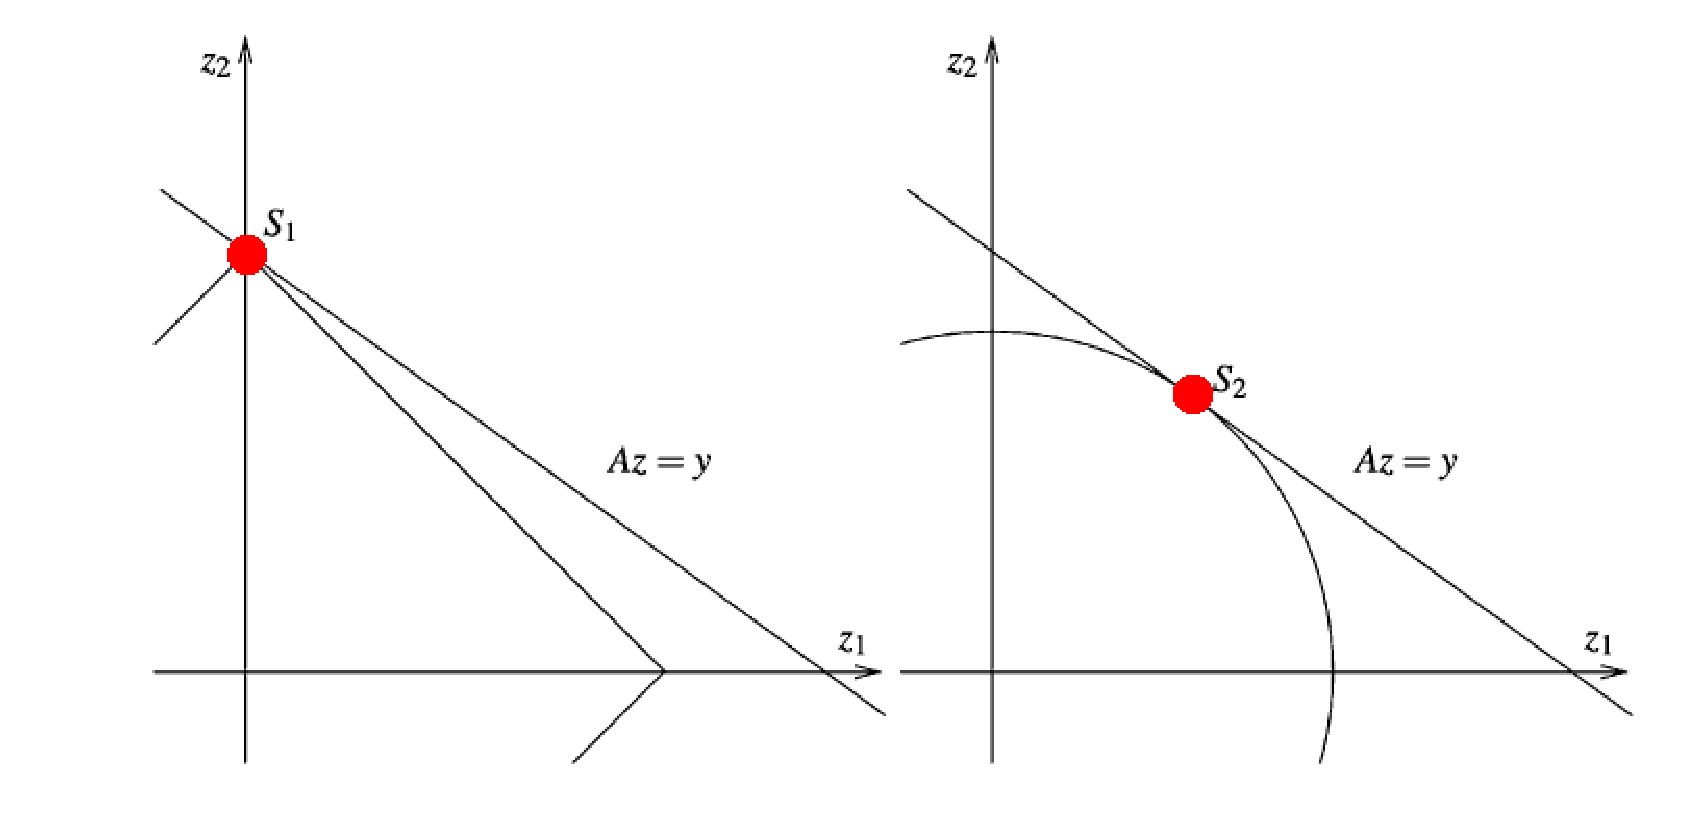
\includegraphics[scale=0.3]{Images/ch1/fig2.eps}
\caption{توپ واحد نُرم مراتب مختلف}
\label{fig2}
\end{figure}






 از روش‌های جایگزین جهت بازیابی سیگنال تنک می‌توان به روش‌های حریص
\LTRfootnote{Greedy}
همانند 
\lr{OMP}\LTRfootnote{Orthogonal Matching Pursuit}
و روش‌های مبتنی بر آستانه‌گذاری مثل 
\lr{IHT}\LTRfootnote{Iterative Hard Thresholding}
اشاره نمود. می‌توان نشان داد که با فرض مناسب، با استفاده از تمامی روش‌های فوق می‌توان سیگنال تنک را بازیابی نمود 
\cite{foucart2013mathematical}.


طراحی ماتریس نمونه‌برداری
$\bm{A}$
یک مساله‌ی جذاب در حسگری فشرده است و به عنوان یک مساله باز، بسیاری از محققان به دنبال تعیین یک ماتریس معین هستند که تمامی قید‌های حسگری فشرده را اقناع کند. برخی از ماتریس‌های معین برگرفته از تئوری تخمین تنک و کدینگ،‌ تا حد مناسبی شرایط بازیابی صحیح را برآورده می‌کنند ولی این ماتریس‌ها از باند بهینه تا حد قابل ملاحظه‌ای دور هستند. خوشبختانه با استفاده از ماتریس‌های تصادفی، شرایط مورد نیاز بازیابی صحیح برآورده می‌گردد. به عنوان دو مثال ساده، می‌توان به ماتریس تصادفی با درایه‌های نرمال و مستقل و یا ماتریس برنولی\LTRfootnote{Bernoulli}
اشاره نمود.
نتایج کلیدی در حسگری فشرده نشان می‌دهد که با احتمال بالا با استفاده از ماتریس تصادفی گوسی یا برنولی
$\bm{A}\in \R^{m \times N}$
، یک بردار 
$s$-تنک
$\bm{x}$
، با استفاده از نمونه‌برداری به صورت
$\bm{y}=\bm{A}\bm{x}$
با تعداد نمونه‌ی 
\begin{align}
\label{eq:eq4}
m \geq C s \log(N/s)
\end{align}
قابل بازیابی است. در عبارت فوق 
$C > 0$
یک مقدار حقیقی ثابت بوده و اثبات شده است که باند محاسبه شده بهینه است
\cite{foucart2013mathematical}.


با توجه به رابطه‌ی
\eqref{eq:eq4}
تعداد نمونه‌ی لازم جهت بازیابی یک سیگنال
$s$-تنک
با 
$s$
رابطه‌ی خطی دارد در صورتی که بعد سیگنال
$N$
، به صورت لگاریتمی با تعداد نمونه در ارتباط است. در صورتی که مقدار 
$s$
بسیار از مقدار
$N$
کوچکتر باشد، تعداد نمونه‌ها در مقایسه با بعد بردار مجهول کم می‌گردد و بازیابی سیگنال با استفاده از سیستم معادلات خطی فرومعین امکان‌پذیر خواهد بود
\cite{candes2006robust}. 


یکی دیگر از خصوصیات مهم در حسگری فشرده 
\textbf{پایداری}
است. به عبارت دیگر در زمانی که نمونه‌های دریافتی کمی غیر دقیق باشند و یا سیگنال مورد بررسی به صورت کامل تنک نباشد، خطای بازیابی  محدود و قابل کنترل است. در این شرایط با حل مساله‌ی کمینه‌سازی نُرم یک درجه‌ی دوم زیر، می‌توان پاسخ را پیدا نمود
\cite{foucart2013mathematical}.
\begin{align}
\label{eq:eq5}
\min \norm{\bm{z}}_{1} \quad \text{s.t.} \quad \norm{\bm{A}\bm{z}-\bm{y}}_{2} \leq \eta
\end{align}
در رابطه‌ی 
\eqref{eq:eq5}
،
$\eta$
برابر با توان نویز جمع‌شونده با سیگنال است.

بدون فرض پایداری، مساله‌ی حسگری فشرده قابل استفاده در کاربرد‌های عملیاتی نخواهد بود. زیرا در بسیاری از کاربرد‌ها، وجود نویز اجتناب‌ناپذیر است. در ادامه به بررسی مساله‌ی حسگری فشرده در حالت کوانتیزه
\LTRfootnote{Quantized}
می‌پردازیم.
%%%%%%%%%%%%%%%%%%%%%%%%%%%%
%%%%%%%%%%%%%%%%%%%%%%%%%%%%
%%%%%%%%%%%%%%%%%%%%%%%%%%%%
\section{حسگری فشرده‌ی کوانتیزه}
در سیستم‌های عملیاتی نمونه‌های دریافتی نمی‌توانند دقت بی‌نهایت داشته باشند و باید به یک الفبا با تعداد عناصر محدود نگاشته گردند.
در کاربرد های عملی هر نمونه (که ممکن است شامل بی نهایت هم باشد) به تعداد محدود و گسسته از مقادیر با دامنه‌ی محدود نگاشته گردد.  برای مثال اگر از یک سیستم کوانتایزر یکنواخت
\LTRfootnote{Uniform quantizer}
با 
$ B $
بیت در هر اندازه‌گیری استفاده کنیم، مقادیر به یکی 
$ 2^B $
مقدار گسسته نگاشته می‌شوند. باید توجه داشت که کوانتیزه کردن نمونه‌ها یک عمل برگشت‌ناپذیر است و همواره مقداری از اطلاعات در این فرآیند از بین می‌رود. 

مشوق اصلی در بررسی حسگری فشرده در حالت کوانتیزه، محدودیت‌های سخت‌افزاری در سیستم‌های دیجیتال است. 
در سیستم‌های سخت‌افزاری یکی از محدودیت‌های اساسی در  مبدل آنالوگ به دیجیتال
(\lr{ADC})
رخ می‌دهد. به عبارت دیگر مبدل آنالوگ به دیجیتال که وظیفه‌ی نمونه‌برداری و کوانتیزه کردن سیگنال ورودی را بر عهده دارد با محدودیت‌های زیر رو به رو است.
\begin{itemize}
\item{
\textbf{سرعت نمونه برداری:}
فرآیند کوانتیزاسیون حداکثر سرعت
\lr{ADC}
را به شدت محدود می‌کند. به طوری که اگر تعداد بیت‌های 
\lr{ADC}
به صورت خطی افزایش یابد، سرعت نمونه‌برداری به صورت نمایی کاهش می‌یابد.
}
\item{
\textbf{هزینه:}
با افزایش تعداد بیت در
\lr{ADC}
هزینه ساخت بالا می‌رود.
}
\item{
\textbf{اثرات غیرخطی}
با افزایش تعداد بیت ساخت قطعات الکترونیکی با اعوجاج کم سخت‌تر می‌شود.
}
\end{itemize}


با توجه به موارد ذکر شده در بالا اگر بتوان تعداد بیت‌های اندازه‌گیری را کاهش داد، به سخت‌افزار‌های بهتر و سریع تری دسترسی داریم
\cite{laska2012regime}.
یکی دیگر از محدودیت‌های عملی در سیستم‌های کاربردی نرخ انتقال داده است. در این سیستم‌ها معمولا چندین بخش مختلف نیاز به ارتباط با یکدیگر دارند که نرخ انتقال اطلاعات بین آنها محدود است. 

در ادامه اثر تعداد بیت و نرخ نمونه‌برداری در خطای بازیابی بررسی شده است.


\section{مدل حسگری فشرده کوانتیزه}
با فرض اینکه سیستم به صورت یکنواخت از سیگنال ورودی نمونه بردارد و تعداد بیت در هر نمونه ثابت فرض شود، می‌توان نرخ حاصل از نمونه‌برداری را به صورت 
$ \mathfrak{B}=mB $
بیان نمود.  
$ \mathfrak{B}$
در واقع نشان‌دهنده‌ی پهنای باند در اختیار جهت انتقال داده‌ها یا  بودجه بیت
\LTRfootnote{Bit budget}
است و در آن 
$m$
برابر با تعداد نمونه‌ها و 
$B$
تعداد بیت در هر نمونه است.
 مدل نمونه‌برداری خطی
\eqref{eq:eq1}
 با اضافه شدن قیود عملی به صورت 
\eqref{eq:eq6}
بیان می‌شود.
\begin{align}
\label{eq:eq6}
\bm{y}_{\mathcal{Q}} =A(\bm{x}):= \mathcal{Q}_{B}\left(\bm{A}(\bm{x}+\bm{n})+\bm{e}\right)
\end{align}
در عبارت فوق ‍
$\bm{n}$
و
$\bm{e}$
به ترتیب نویز قبل و بعد از نمونه‌برداری و
$\mathcal{Q}_{B}$
تابع کوانتایزر 
$B$
بیتی که مقادیر حقیقی نمونه‌های حسگری فشرده را به الفبای گسسته‌ی 
$\mathfrak{U}$
با 
$2^{B}$
عضو می‌نگارد. در این بخش بردار
$\bm{n}$
به صورت یک بردار تصادفی که هر درایه‌ی آن از توزیع نرمال با میانگین صفر و واریانس
$\sigma_{\bm{n}}^{2}$
 است، انتخاب شده است. همچنین مقدار
$\norm{\bm{e}}_{2}$
را برابر با صفر در نظر می‌گیریم.


با فرض 
$ \mathfrak{B}$
و نویز ثابت، کارایی سیستم را می‌توان بر اساس تعداد نمونه‌ها بررسی نمود. از طرف دیگر، با توجه به اینکه 
$B = \mathfrak{B}/m$
است،‌ می‌توانیم با کاهش تعداد نمونه‌ها، تعداد بیت در هر نمونه را افزایش دهیم که منجر به افزایش دقت در هر نمونه می‌گردد. بنابراین اگر ما تعداد نمونه‌ی کمتری برداریم، می‌توانیم به هر نمونه تعداد بیت بیشتری اختصاص دهیم ولی در اثر نویز ممکن است با اخذ هر نمونه تعداد بیت بیشتری حامل داده‌های غلط باشند.

در مرجع
\cite{laska2012regime}
با فرض نویز مستقل و گوسی تعداد بیت بهینه که متوسط مربع خطا
\LTRfootnote{MSE}
را کمینه می‌کند طبق رابطه‌ی 
\eqref{eq:eq7}
به دست آمده است.
\begin{align}
\label{eq:eq7}
B \approx \dfrac{1}{2}\log_{2}\left( \dfrac{\norm{\bm{x}}_{2}^{2}}{\sigma^{2}_{\bm{n}}}\dfrac{m}{N}\right)
\end{align}

با فرض نمونه‌برداری یکنواخت و
$ \mathfrak{B} $
ثابت معادله‌ی فوق را می توان به صورت زیر بازنویسی کرد.
\begin{align}
\label{eq:eq8}
\log_{2}\left( \dfrac{\norm{\bm{x}}_{2}^{2}}{N \sigma^{2}_{\bm{n}}}\right)\approx \dfrac{2\mathfrak{B}}{m}-\log_{2}\left(m\right)
\end{align}

عبارت سمت چپ بیانگر نسبت سیگنال به نویز
(\lr{SNR})
است. با توجه به 
\eqref{eq:eq7}
سیگنال را در دو حالت مختلف می‌توان بررسی کرد.
\begin{itemize}
\item{
\textbf{سیگنال‌های قوی:}
در این حالت سمت چپ عبارت عدد بیشتری دارد بنابراین برای حداقل شدن خطا باید تعداد اندازه گیری‌ها کم و تعداد بیت در هر اندازه‌گیری بالا باشد. 
}
\item{
\textbf{:سیگنال‌های ضعیف}
در این حالت بر خلاف حالت قبلی بهتر است از تعداد نمونه‌های بیشتر با تعداد بیت کمتر در هر نمونه استفاده شود.
}
\end{itemize}

\section{باند خطا}
در مرجع
\cite{laska2012regime}
یک باند خطا برای سیستم نمونه برداری شده به صورت زیر بدست آمده است.
\begin{theorem}
\label{thorem:thm1}
فرض کنید، 
$\bm{y}_{\mathcal{Q}} =A(\bm{x}):= \mathcal{Q}_{B}\left(\bm{A}(\bm{x}+\bm{n})\right)$
و سیگنال
$\bm{x}\in \R^N$
دارای  پشتیبان
$\Omega \in \lbrace 1,\cdots,N\rbrace$
با اندازه‌ی 
$|\Omega|=s$
باشد. درایه‌های 
$\Omega$
به صورت تصادفی با توزیع یکنواخت و دامنه‌ی عناصر غیر صفر به صورت 
$ x_{i} \in \Omega \sim \mathcal{N}\left( 0,\sigma_{\bm{x}}^{2} \right) $
بدست آمده‌اند. درایه‌های بردار نویز
$\bm{n}\in \R^m$ 
به صورت تصادفی از توزیع نرمال با میانگین صفر و واریانس
$\sigma^{2}_{\bm{n}}$
انتخاب شده است. همچنین فرض کنید که درایه‌های ماتریس نمونه‌برداری
$\bm{A}\subset \R^{m\times N}$
در شرط 
\lr{RIP}\LTRfootnote{Restricted Isometry Property}
از مرتبه‌ی
$s$
و ثابت
$\delta$
صدق کند. با انتخاب مناسب 
$\mathcal{Q}$
 و مقدار ثابت 
$\mathfrak{B}=mB$
، مقدار 
\lr{MSE}
در شرط زیر صدق خواهد کرد.
\begin{align}
\label{eq:eq9}
\mathbb{E}\left( \norm{\bm{x}-\hat{\bm{x}}}_{2}^{2} \right) \leq \dfrac{2s}{\mathfrak{B}\left( 1-\delta\right)} \left[ s\sigma^{2}_{\bm{x}}B2^{-2B}+N\sigma^{2}_{\bm{n}}B\left(1+2^{-2B}\right)\right]\\ \nonumber
\qquad \qquad+\dfrac{s}{\left( 1-\delta\right)}\left(\dfrac{\mathfrak{B}}{B}-1\right)\mathfrak{S}
\end{align}
که در آن 
$ \mathfrak{S}=\max_{i\neq j}\vert \mathbb{E}\mathcal{Q}_{B}\left(\bm{A}(\bm{x+n})\right)_{i}\mathcal{Q}_{B}\left(\bm{A}(\bm{x+n})\right)_{j}\vert $
است.
\end{theorem}
\begin{proof}
 این قضیه در 
\cite{laska2012regime}
اثبات شده است.
\end{proof}
در معادله مذکور عبارت 
$ s\sigma^{2}_{\bm{x}}B2^{-2B} $
بیانگر خطای ناشی از کوانتیزاسیون سیگنال و عبارت 
$ N\sigma^{2}_{\bm{n}}B\left(1+2^{-2B}\right) $
اثر نویز و کوانتیزاسیون را به صورت همزمان نشان می‌دهد. عبارت 
$ \left(\dfrac{\mathfrak{B}}{B}-1\right)\mathfrak{S} $
نشان دهنده‌ی اثر همبستگی در اندازه گیری کوانتیزه شده است.

در بسیاری از سناریو‌های حسگری فشرده، انتظار داریم که مقدار عبارت آخر در سمت راست رابطه‌ی 
\eqref{eq:eq9}
به صفر میل کند. برای مقادیر بزرگ 
$B$
، در مرجع 
\cite{gray1998quantization}
نشان داده شده است که این عبارت با تقریب خوبی به صفر میل می‌کند. بنابراین انتخاب مقدار بهینه‌ی 
$B$
با متعادل‌سازی دو عبارت داخل کروشه بستگی دارد. 

باند خطای محاسبه شده در رابطه‌ی 
\eqref{eq:eq9}
برای سیگنال‌های تنک کامل به دست آمده است. در صورتی که دسته‌ی مهم دیگری از سیگنال‌ها در پردازش سیگنال دیجیتال، سیگنال‌های فشرده‌پذیر هستند. در سیگنال‌های فشرده‌پذیر قسمت عمده‌ی توان در 
$s$
مولفه از سیگنال به ترتیب نزولی دامنه، قرار دارد. در این حالت 
$N-s$
مولفه‌ی دیگر را دنباله‌ی سیگنال می‌نامیم. برای چنین سیگنالی، دنباله‌ی سیگنال همانند نویز فرض می‌شود و در فرآیند بازیابی حذف می‌گردد
\cite{davenport2012pros,davies2011sample}.
نتایج قضیه‌ی
\ref{thorem:thm1}
را می‌توان به سیگنال‌های فشرده‌پذیر تعمیم داد. در این حالت مقادیر کوچک و غیر صفر به صورت نویز مدل می‌شوند.



برای مقایسه‌ی اثر توان سیگنال و تعداد بیت دو پارامتر 
\lr{ISNR}\LTRfootnote{Input SNR}
و
\lr{RSNR}\LTRfootnote{Reconstruction SNR}
را به صورت زیر تعریف می‌کنیم.
\begin{align}
\label{eq9}
ISNR := 10\log_{10}\left( \dfrac{\mathbb{E}\left( \norm{\bm{x}}_{2}^{2} \right)}{\mathbb{E}\left( \norm{\bm{n}}_{2}^{2} \right)} \right)
\end{align}
\begin{align}
\label{eq10}
RSNR := 10\log_{10}\left( \dfrac{\norm{\bm{x}}_{2}^{2}}{\norm{\bm{x}-\bm{x}^{\star}}_{2}^{2}} \right)
\end{align}

در شکل
\ref{fig3}
مقدار 
\lr{MSE}
به ازای 
\lr{ISNR}های
مختلف نشان داده شده است.
\begin{figure}[H]
\centering
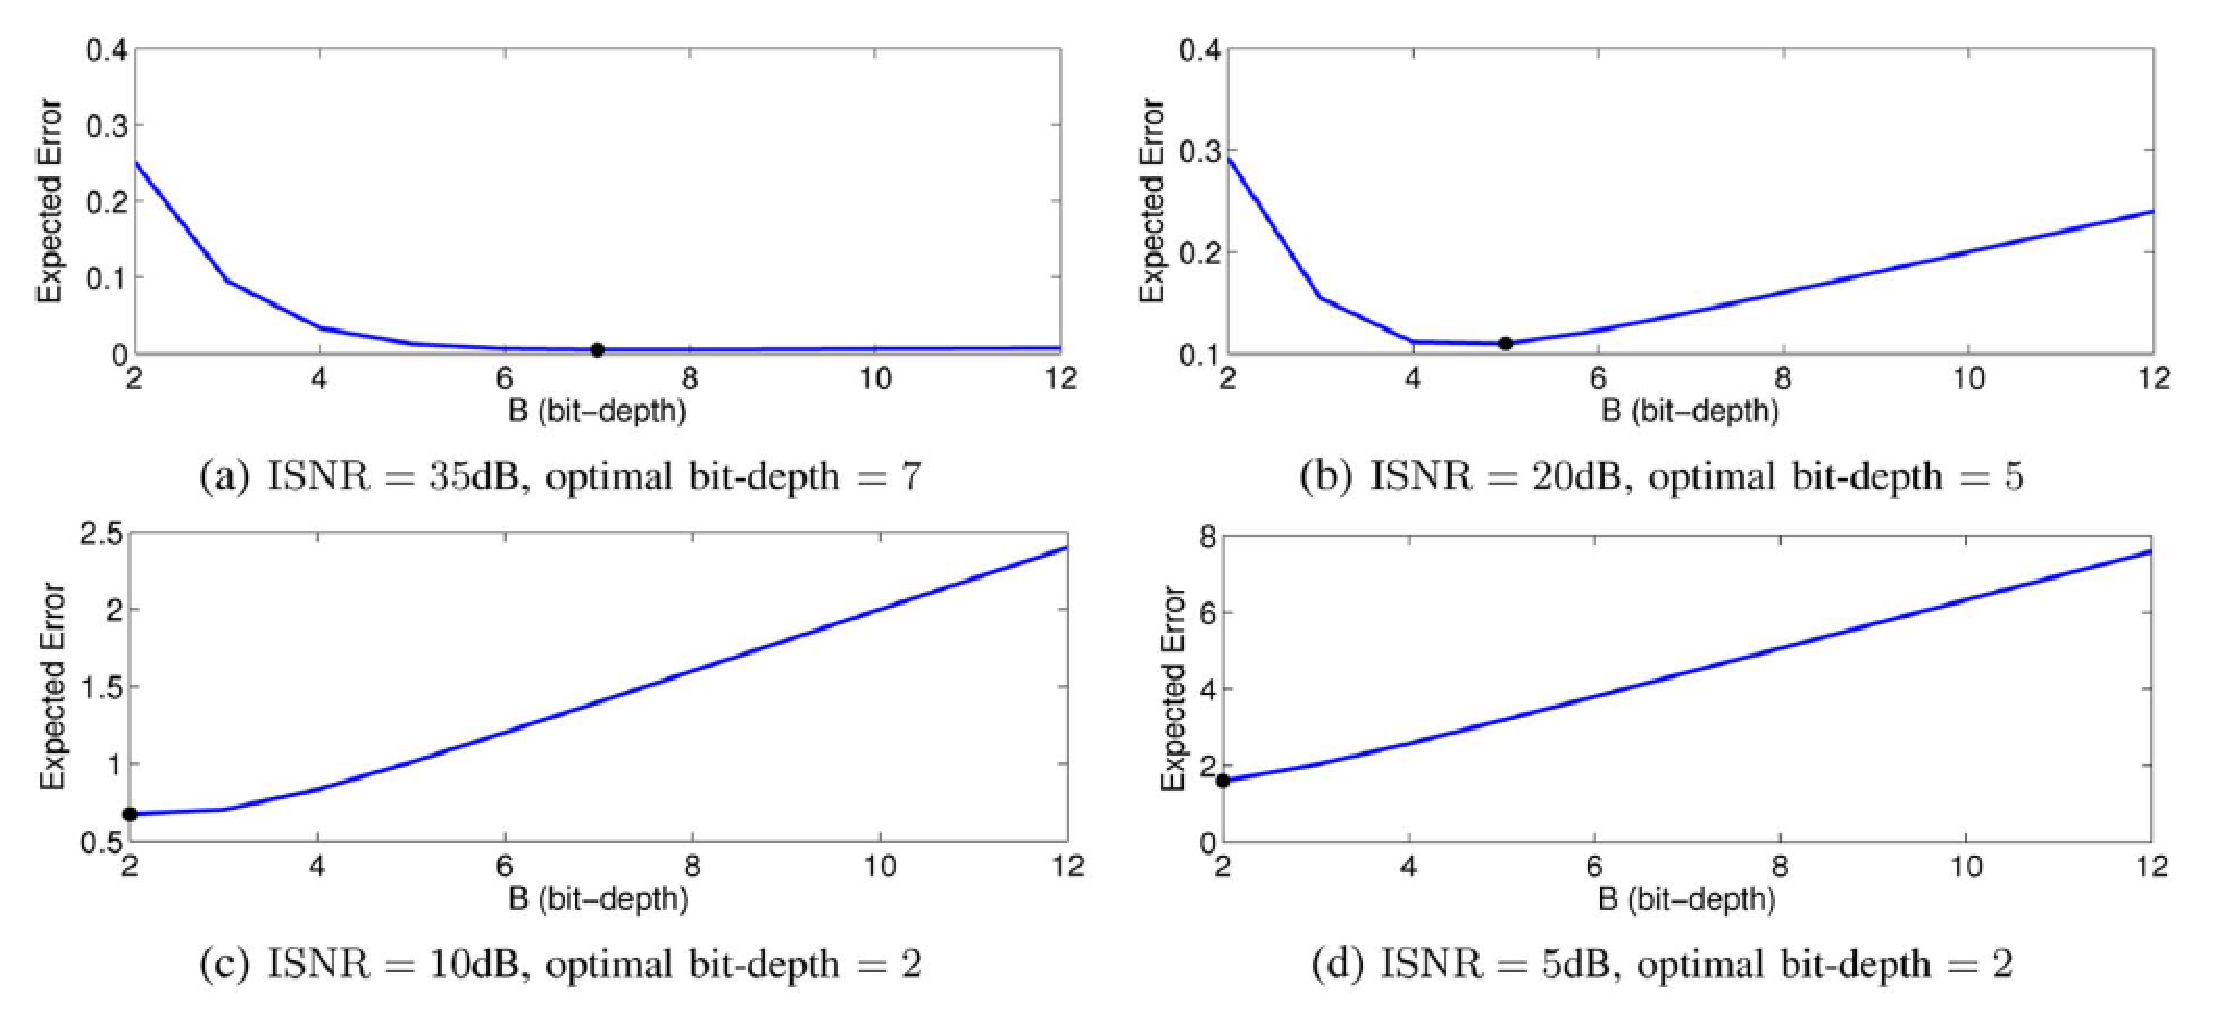
\includegraphics[scale=0.34]{Images/ch1/fig3.eps}
\caption{مقدار 
\lr{MSE}
به ازای 
\lr{ISNR}های
مختلف\cite{laska2012regime} }
\label{fig3}
\end{figure}

با توجه به شکل برای سیگنال‌های قوی تعداد بیت بیشتر و برای سیگنال‌های ضعیف تعداد بیت کمتر منجر به کاهش خطا می‌گردد.
نکته‌ی قابل توجه در این نمودار رفتار خطا به ازای افزایش تعداد بیت است. همان‌گونه که مشخص است در همه‌ی حالات تعداد بیت بالا لزوما بهینه نیست. علاوه بر این، همانگونه که انتظار داشتیم، حداقل خطای بازیابی به ازای 
\lr{ISNR}
پایین، در تعداد بیت کم رخ می‌دهد.

به عنوان یک نتیجه‌ی کلی می‌توان گفت که در صورتی که سیگنال مورد بررسی دارای نسبت سیگنال به نویز پایین باشد، با تعداد بیت کم نیز می‌توان سیگنال را بازیابی نمود.
\section{حسگری فشرده تک بیتی}
بررسی‌ها بر روی محدودیت تعداد بیت در هر نمونه نشان داد که تنها یک بیت در هر نمونه از سیگنال جهت بازیابی صحیح سیگنال کافی است
\cite{boufounos20081} .
در این حالت مدل نمونه‌برداری از بردار 
$\bm{x}$
به صورت رابطه‌ی 
\eqref{eq:eq10}
خواهد بود.
\begin{align}
\label{eq:eq10}
\bm{y}= \text{sign}\left(\bm{A}\bm{x}\right).
\end{align}


نمونه‌برداری تک بیتی در  مسایل آماری و مهندسی کاربرد دارد. از کاربرد‌های نمونه‌برداری تک بیتی ‌می‌توان به موارد زیر اشاره نمود.
\begin{itemize}
\item{
\textbf{
بازیابی سیگنال و مبدل‌های آنالوگ به دیجیتال.
}
وظیفه‌ی یک مبدل آنالوگ به دیجیتال نمونه‌برداری از سیگنال آنالوگ
$ \bm{x} $
و به دست آوردن تقریب دیجیتال
$ \widehat{\bm{x}}$
است. در صورتی که سیگنال تنک باشد، تعداد نمونه‌ها کاهش می‌یابد. در عمل تعداد بیت بالا در سخت‌افزار منجر به گران‌تر شدن سخت‌افزار می‌شود ولی نمونه‌برداری تک بیتی به معنای یک مقایسه کننده است که پیاده‌سازی آسان و ارزان دارد. 
}
\item{
\textbf{
رگرسیون دودویی.
}\LTRfootnote{Binary regression}
در یکی از مدل‌های رگرسیون منطقی، فرآیند تصمیم‌گیری یک فرد را با بردار
$ \bm{a}_{i} $
و پاسخ فرد در مورد یک موضوع را با بردار
$ \bm{x} $
نشان می‌دهند. اگر 
$ \langle \bm{a}_{i}  , \bm{x}\rangle > \nu_{i} $
باشد، پاسخ مثبت و در غیر این صورت پاسخ منفی است. در رگرسیون دودویی تنک همانند حسگری فشرده هدف پیدا کردن 
$ \bm{x} $
است. بنابراین از نتایج حسگری فشرده تک بیتی می‌توان در این حوزه نیز استفاده نمود.
}
\item{
\textbf{
الگوریتم‌های پخش عمومی.
}\LTRfootnote{Streaming algorithms and broadcasting }
فرض کنید گره‌ی مرکزی\LTRfootnote{Centeral node}
فایل 
$ \bm{x} $
را دارد (که به صورت تنک مدل شده است) و می‌خواهد به یک یا چند گره که هرکدام  دقت متفاوت دارند، ارسال کند. یک گزینه پخش عمومی بیت‌های
$ \text{sign}\left( \langle \bm{a}_{i}  , \bm{x}\rangle - \nu_{i}  \right) $
است. گره‌های مقصد با توجه به دقت و سایر مشخصات خود و کانال، تعداد بیت لازم جهت بازیابی صحیح را دریافت می‌کند.
}
\end{itemize}

از طرف دیگر در بعضی مواقع با توجه به محدودیت در پهنای باند، توان و یا هزینه‌ی عملیاتی سیستم، استفاده از نمونه‌های تک بیتی تنها گزینه‌ی موجود است. به عنوان مثال می‌توان به برخی از گیرنده‌های دیجیتال باند وسیع یا سیستم‌های انبوه آنتنی
\LTRfootnote{Massive MIMO}
اشاره نمود
\cite{Yin2010,risi2014massive,jacques2013robust, baraniuk2017exponential}.


با فرض نمونه‌برداری به صورت
\eqref{eq:eq10}
بردار
$\bm{y}$
هیچ اطلاعاتی از دامنه‌ی بردار
$\bm{x}$
ندارد و در این حالت ما امیدواریم که تنها بتوانیم جهت بردار 
$\bm{x}$
را تخمین بزنیم. خوشبختانه، اگر با تغییر در مدل نمونه‌برداری، بجای آستانه‌ی صفر از آستانه‌های تصادفی (به عنوان مثال 
$\tau_{i} \sim \mathcal{N}(0,1)$
) برای هر نمونه استفاده گردد، اطلاعات دامنه‌ی سیگنال حفظ می‌شود. در این حالت مدل نمونه‌برداری به صورت 
\eqref{eq:eq11}
تغییر خواهد کرد.
\begin{align}
\label{eq:eq11}
\bm{y}= \text{sign}\left(\bm{A}\bm{x}-\bm{\tau}\right).
\end{align}
در بخش‌های آتی تفاوت بین دو رابطه‌ی 
\eqref{eq:eq10}
و  
\eqref{eq:eq11}
از دیدگاه هندسی بررسی شده است.


بخش عمده‌ای از تحقیقات در حسگری فشرده صرف بازیابی سیگنال‌های تنک شده است. در صورتی که بسیاری از سیگنال‌های طبیعی بعد از یک تبدیل تنک می‌گردند. به عنوان مثال سیگنال‌های سینوسی در فضای فوریه تنک هستند و یا تصاویر پس از تبدیل ویولت
\LTRfootnote{Wavelet}
تنک می‌گردند. در صورتی که از یک تبدیل متعامد استفاده کنیم، نتایج حسگری فشرده به سادگی قابل تعمیم به این حوزه خواهد بود. از سوی دیگر، دسته‌ای از سیگنال‌ها که دیکشنری-تنک نامیده می‌شوند، در یک دیکشنری غیر متعامد تنک هستند. برای مثال  سیگنال‌های رادار در چارچوب گابور
\LTRfootnote{Gabor frame}
تنک هستند. مساله‌ی دیکشنری‌های افزونه
\LTRfootnote{Redundant dictionary}
ابتدا در مرجع 
\cite{Candes2011}
بررسی شد و در ادامه در
\cite{Baraniuk2017}
به حسگری فشرده تک بیتی گسترش داده شده است.

\section{کار‌های قبلی}
در این بخش، کارهای انجام شده در زمینه‌ی حسگری فشرده‌ی تک بیتی به صورت مختصر مرور شده است.
در حسگری فشرده سنتی، نمونه‌ها به صورت اعداد اسکالر فرض می‌شدند. نویسندگان
\cite{boufounos20081}
مدل نمونه‌برداری را تغییر دادند و فرض کردند که تنها علامت مشاهدات در دسترس است. بر همین مبنا، الگوریتم بازیابی سیگنال را طراحی کردند. در 
\cite{laska2012regime}،
اثر تعداد بیت در هر نمونه برای سیگنال‌های قوی و ضعیف بررسی گردید و  استفاده از تعداد بیت کم در حالتی که سیگنال ورودی دارای نسبت سیگنال به نویز پایین است را پیشنهاد داد. در این میان تعداد زیادی الگوریتم جدید طراحی گردید که به عنوان مثال می‌توان به 
\lr{Matching Sign Pursuit (MSP)}،
\lr{Restricted-Step Shrinkage (RSS)}
و
\lr{Binary Iterative Hard Thresholding (BIHT)}
اشاره نمود
\cite{boufounos2009greedy,laska2011trust,jacques2013robust}.


در  
\cite{jacques2013robust}،
یک باند بالا برای خطای بازیابی بر اساس درجه تنکی و تعداد نمونه‌ها محاسبه گردید. 	علاوه بر این، معیار 
\lr{B$\epsilon$SE}
را برای ماتریس اندازه‌گیری معرفی نمود. این معیار مشابه معیار 
\lr{RIP}
در حسگری فشرده سنتی است. 

در ادامه نویسندگان
\cite{plan2013one}
، مساله‌ی حسگری فشرده‌ی تک بیتی را از دیدگاه هندسی بررسی کردند و یک پاسخ بهینه برای مساله‌ی حسگری فشرده تک بیتی ارائه دادند. در ادامه در 
\cite{plan2013robust}
حالت نویزی مساله نیز بررسی گردید.

در 
\cite{knudson2016one}
دو الگوریتم جهت بازیابی کامل سیگنال (اندازه و جهت)‌ ارائه گردید.  الگوریتم اول از آستانه‌های تصادفی جهت بازیابی سیگنال استفاده می‌کند و در الگوریتم دوم اندازه و جهت سیگنال به صورت جداگانه به دست می‌آیند. در 
\cite{kamilov2012one}
یک الگوریتم وفقی با استفاده از 
\lr{GAMP\LTRfootnote{Generalized approximate message passing algorithm}}
طراحی گردید که در آن آستانه‌ها در طول زمان نمونه‌برداری به روز می‌گردند.

با این وجود، تحقیقات گسترده‌ای به همراه الگوریتم‌های مختلف جهت کاهش خطای بازیابی در حسگری فشرده‌ی تک بیتی طراحی گردید.  در  
\cite{Guentuerk2003}
، از کوانتایزر تک بیتی سیگما-دلتا جهت رسیدن به نرخ کاهش نمایی استفاده گردید. در  
\cite{baraniuk2017exponential}،
با استفاده از همین رویکرد، یک سناریوی نمونه‌برداری و بازیابی وفقی طراحی شده است که با استفاده از آن می‌توان به نرخ کاهش نمایی  در حسگری فشرده‌ی تک بیتی دسترسی پیدا نمود.

کار جدید بارانیوک
\LTRfootnote{Baraniuk}
و همکاران، نشان داد که با استفاده از الگوریتم مبتنی بر بهینه‌سازی محدب و یا آستانه‌گذاری می‌توان اندازه و جهت سیگنال‌های دیکشنری-تنک را بازیابی نمود
\cite{Baraniuk2017}.

در این پایان‌نامه، ما از آستانه‌گذاری وفقی برای بازیابی سیگنال‌های دیکشنری تنک استفاده نموده‌ایم و جهت اثبات مباحث هندسه‌ی ابعاد بالا بکار رفته است.

\section{نشانه‌گذاری}
در این قسمت، نشانه‌گذاری مورد استفاده در پایان‌نامه بیان شده است.
بردار‌ها و ماتریس‌ها به ترتیب با حروف کوچک و بزرگ توپر نشان داده شده است. 
 $ \bm{v}^T $ 
 و
 $ \bm{v}^{\ast} $
به ترتیب نشان‌دهنده‌ی عملیات انتقال و مزدوج-انتقال بردار 
$ \bm{v} $
است. مقادیر مثبت، صحیح و ثابت با حروف بزرگ و کوچک لاتین نشان داده شده است که ممکن است خط به خط تغییر کند.
مقدار نُرم 
$\ell_2$ 
بردار
$ \bm{v} \in \R^n $
به صورت
$ \norm{\bm{v}}_2= \sqrt{\Sigma_i v_i^2} $
و نُرم 
$\ell_1$ 
به صورت
 $ \norm{\bm{v}}_1= \Sigma_i |v_i|$
و نُرم
$ \ell_{\infty} $
به صورت
$ \norm{\bm{v}}_{\infty}= \max_{i} |v_{i}| $
 تعریف می‌گردد.
  $ \norm{\bm{v}}_0 $
 نشان‌دهنده‌ی تعداد عناصر غیر صفر بردار
 $ \bm{v} $
 است و اگر
 $ \norm{\bm{v}}_0 \leq s$
 باشد،  بردار را
$s$-تنک
می‌نامیم. 
$ B_1^n := \{\bm{v}\in \R^n : \norm{\bm{v}}_{1}\leq 1 \} $ 
برابر با توپ $ \ell_1 $، 
$ B_2^n := \{\bm{v}\in \R^n : \norm{\bm{v}}_{2}\leq 1 \} $
برابر با توپ $ \ell_2 $ و 
$ S^{n-1}:= \{\bm{v}\in \R^n : \norm{\bm{v}}_{2}= 1 \} $
نشانگر کره واحد اقلیدسی است.
در طول این پایان‌نامه،
 $ d_{G}\left(\bm{v},\bm{u}\right):=1/\pi \arccos\langle \bm{v},\bm{u} \rangle $
نشانگر فاصله‌ی نرمالیزه‌ی ژئودزیک
\LTRfootnote{Normalized geodesic distance}
بین دو بردار 
$ \bm{u} $
و
$ \bm{v}$
روی 
$ S^{n-1} $ 
است. 

\section{طرح کلی}

در فصل
\ref{ch:HDE}
رویکرد هندسی در حوزه‌ی آشکارسازی و ابزارها به همراه مثال ارائه گردیده است. در ادامه مدل بیان شده به حسگری فشرده تعمیم یافته است.
پس از بیان مقدمات و ابزار‌های مورد نیاز جهت تحلیل موضوع به صورت هندسی، در ابتدای فصل
\ref{ch:main}
مساله‌ی سیگنال‌های دیکشنری تنک بررسی شده است. در این بخش ابتدا اهمیت سیگنال‌های دیکشنری تنک بیان گردیده و در ادامه به بیان چارچوب ریاضی آن پرداخته‌ایم.
در ادامه با بیان مدل سیستم مورد بررسی و همچنین تعاریف مورد نیاز الگوریتم پیشنهادی جهت بازیابی سیگنال دیکشنری تنک با استفاده از نمونه‌های تک بیتی ارائه شده و سپس، تحلیل تئوری و ضمانت‌های ریاضی الگوریتم بیان گردیده است.

در انتها، در فصل آخر، تنایج شبیه‌سازی الگوریتم پیشنهادی به همراه مقایسه با الگوریتم موجود، آورده شده است.

اثبات ریاضی نتایج در پیوست آورده شده است.



